\documentclass[11pt]{article}
\usepackage{amsmath, amssymb, amscd, amsthm, amsfonts}
\usepackage{graphicx}
\usepackage{hyperref}
\usepackage{float}
\usepackage{subfigure}
\usepackage[framed,numbered,autolinebreaks,useliterate]{mcode}

\oddsidemargin 0pt
\evensidemargin 0pt
\marginparwidth 40pt
\marginparsep 10pt
\topmargin -20pt
\headsep 10pt
\textheight 8.7in
\textwidth 6.65in
\linespread{1.2}

\title{Tugas EB3102 - Pengolahan Sinyal Biomedika}
\author{Irfan Tito Kurniawan - 18317019}
\date{23 Desember 2019}

\newtheorem{theorem}{Theorem}
\newtheorem{lemma}[theorem]{Lemma}
\newtheorem{conjecture}[theorem]{Conjecture}

\newcommand{\rr}{\mathbb{R}}

\newcommand{\al}{\alpha}
\DeclareMathOperator{\conv}{conv}
\DeclareMathOperator{\aff}{aff}

\begin{document}

\maketitle

\section{Topik I: Analisis Sinyal}\label{topik-i}
\subsection{Teori}
\subsubsection{Electrocardiogram}

\textit{Electrocardiogram}, selanjutnya disebut dengan \textbf{ECG}, merupakan sinyal listrik yang merepresentasikan aktivitas jantung. ECG merupakan salah satu biosinyal utama yang digunakan untuk membantu proses diagnosis penyakit. Umumnya, sinyal ECG diteliti dalam \textit{domain} waktu, sehingga dibutuhkan sinyal ECG yang bersih dan benar-benar merepresentasikan aktivitas jantung. Akan tetapi, pada kenyataannya, sinyal ECG yang memiliki amplitudo yang relatif kecil terbaca bercampur dengan derau yang kebanyakan memiliki amplitudo lebih besar dibandingkan dengan sinyal ECG. Karena itu, diperlukan proses \textit{filtering} untuk memperoleh sinyal ECG yang bersih dan dapat diandalkan.

\begin{figure}[H]
\centerline{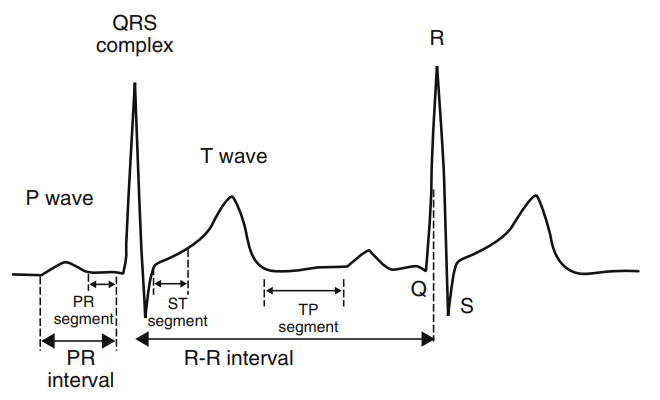
\includegraphics[scale=0.35]{figures/fig2-ecgsegments.png}}
\caption{Sinyal ECG \cite{archarya14}}
\end{figure}

Sinyal ECG dapat dibagi menjadi beberapa segmen: gelombang P, kompleks QRS, serta gelombang T. Tiap segmen memiliki rentang frekuensi sinyal yang berbeda-beda. Dengan transformasi Fourier dari gelombang ECG, didapati bahwa segmen gelombang P-T secara umum memiliki rentang frekuensi sinyal antara 0.5 hingga 10 Hz sedangkan kompleks QRS memiliki rentang frekuensi sinyal antara 4 hingga 20 Hz \cite{thakor84}.

\begin{figure}[H]
\centerline{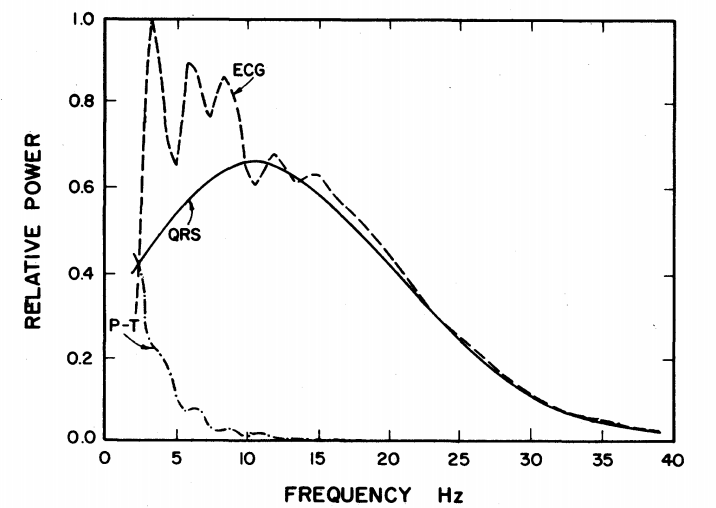
\includegraphics[scale=0.3]{figures/fig1-ecgspectrum.png}}
\caption{Spektrum Frekuensi Sinyal ECG \cite{thakor84}}
\end{figure}

\subsubsection{Derau}
Derau yang mengotori sinyal ECG berasal dari berbagai sumber. Derau tersebut di antaranya: interferensi jala-jala, derau kontak elektroda, artefak akibat gerakan, kontraksi otot, dan pergeseran \textit{baseline} atau dasar sinyal \cite{archarya14}. Tiap jenis derau memiliki rentang frekuensi yang berbeda-beda. Pada laporan ini, derau pada pembacaan sinyal ECG akan dibagi menjadi beberapa jenis, yakni derau akibat interferensi jala-jala, derau yang menyebabkan pergeseran \textit{baseline}, serta derau berfrekuensi tinggi.

Interferensi jala-jala merupakan derau akibat adanya kapasitansi parasitik antara jala-jala dengan tubuh. Karenanya, derau akibat interferensi jala-jala memiliki frekuensi yang sama dengan frekuensi tegangan jala-jala beserta dengan harmonisanya. Sebagai contoh, apabila tegangan jala-jala pada tempat pengukuran sebesar 120 VAC 60 Hz, maka akan muncul derau akibat interferensi jala-jala pada frekuensi 60 Hz, 120 Hz, 180 Hz, begitu seterusnya. Derau jenis ini boleh jadi memiliki frekuensi yang \textit{overlapping} dengan frekuensi informasi sinyal ECG. Untuk menghilangkan derau jenis ini, pada umumnya digunakan \textbf{Notch Filter} atau \textbf{Comb Filter}.

Derau yang menyebabkan pergeseran \textit{baseline} merupakan derau berfrekuensi rendah, pada umumnya memiliki frekuensi DC atau 0 Hz hingga 0.8 Hz \cite{archarya14}. Karenanya, derau jenis ini boleh jadi pula memiliki frekuensi yang \textit{overlapping} dengan frekuensi informasi sinyal ECG. Derau jenis ini dapat disebabkan oleh proses pernapasan dan gerakan subyek. Derau jenis ini dapat dihilangkan dengan \textbf{High-pass Filter} dengan frekuensi \textit{cutoff} rendah.

\begin{figure}[H]
\centerline{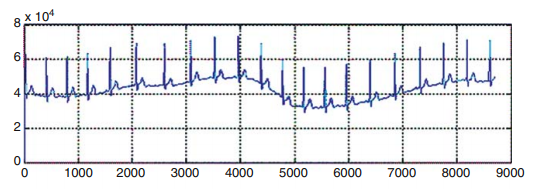
\includegraphics[scale=0.4]{figures/fig3-baselinewander.png}}
\caption{Sinyal ECG dengan Derau Penggeser \textit{Baseline} \cite{thakor84}}
\end{figure}

Kemudian, jenis derau yang ketiga adalah derau berfrekuensi tinggi. Derau jenis ini menyebabkan adanya \textit{jitter} atau fluktuasi cepat sinyal ECG. Derau berfrekuensi tinggi dapat disebabkan oleh kontraksi otot dan derau akibat kontak elektroda yang kurang baik. Derau jenis ini memiliki rentang frekuensi yang sangat lebar, dari dalam rentang frekuensi sinyal ECG hingga di atas frekuensi sinyal ECG. Derau jenis ini dapat dimodelkan sebagai perubahan \textit{baseline} yang terjadi secara cepat dan acak yang meluruh secara eksponensial \cite{archarya14}. Karena itu, selain dapat dihilangkan dengan \textbf{Low-pass Filter} dengan frekuensi \textit{cutoff} tinggi, derau jenis ini juga akan hilang ketika bacaan sinyal dirata-ratakan.

\subsubsection{Analisis Sinyal}
Untuk menghilangkan derau dari sinyal ECG yang ada, pertama kita perlu mengetahui jenis derau yang ada dalam sinyal beserta dengan karakteristiknya. Salah satu cara paling mudah untuk mengetahui jenis dan karakteristik derau dalam sinyal adalah dengan melihat \textit{Power Spectral Density} (PSD) dari sinyal yang diperoleh. PSD dari suatu sinyal menunjukkan bagaimana daya sinyal tersebut tersebar dalam \textit{domain} frekuensi \cite{oppenheim}.

Spektrum daya pada frekuensi $\omega$, $S_{xx}(\omega)$, dari suatu sinyal $x(n)$ yang memiliki transformasi Fourier $X(\omega)$ didefinisikan sebagai
\begin{equation}
    S_{xx}(\omega) = |X(\omega)|^2
\end{equation}
Dengan demikian, PSD dari sinyal $x(n)$ dapat diperoleh dengan melakukan transformasi Fourier pada sinyal tersebut, kemudian mengkuadratkan magnituda spektrum sinyal pada \textit{domain} frekuensi.

Dari persamaan diatas, diturunkan proses analisis sinyal berikut
\begin{figure}[H]
\centerline{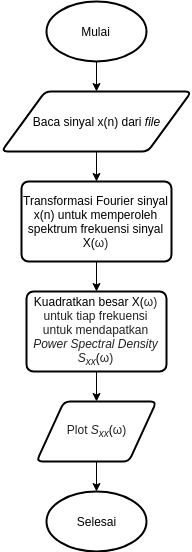
\includegraphics[scale=0.6]{figures/fig4-diagramalirtopik1.png}}
\caption{Diagram Alir Analisis Sinyal}
\end{figure}

\subsection{Hasil dan Pembahasan}
Diberikan dua buah sampel sinyal ECG untuk dianalisis. Selanjutnya, sinyal dalam \textit{file} 'psb\textunderscore ecg1.dat' akan disebut sebagai 'sampel ECG 1' dan sinyal dalam \textit{file} 'psb\textunderscore ecg2.dat' akan disebut sebagai 'sampel ECG 2'. Kedua sinyal ini dianalisis dan ditampilkan sesuai dengan diagram alir pada bagian sebelumnya. Untuk menghitung transformasi Fourier dari kedua sinyal ini, digunakan algoritma \textit{Fast Fourier Transform} (FFT), kemudian PSD dari sinyal dihitung dengan mengkuadratkan tiap spektrum hasil FFT dari sinyal.

Sinyal sampel ECG 1 akan dibahas terlebih dahulu. Berikut adalah plot sinyal sampel ECG 1 dalam \textit{domain} waktu beserta dengan PSD-nya

\begin{figure}[H]
\centerline{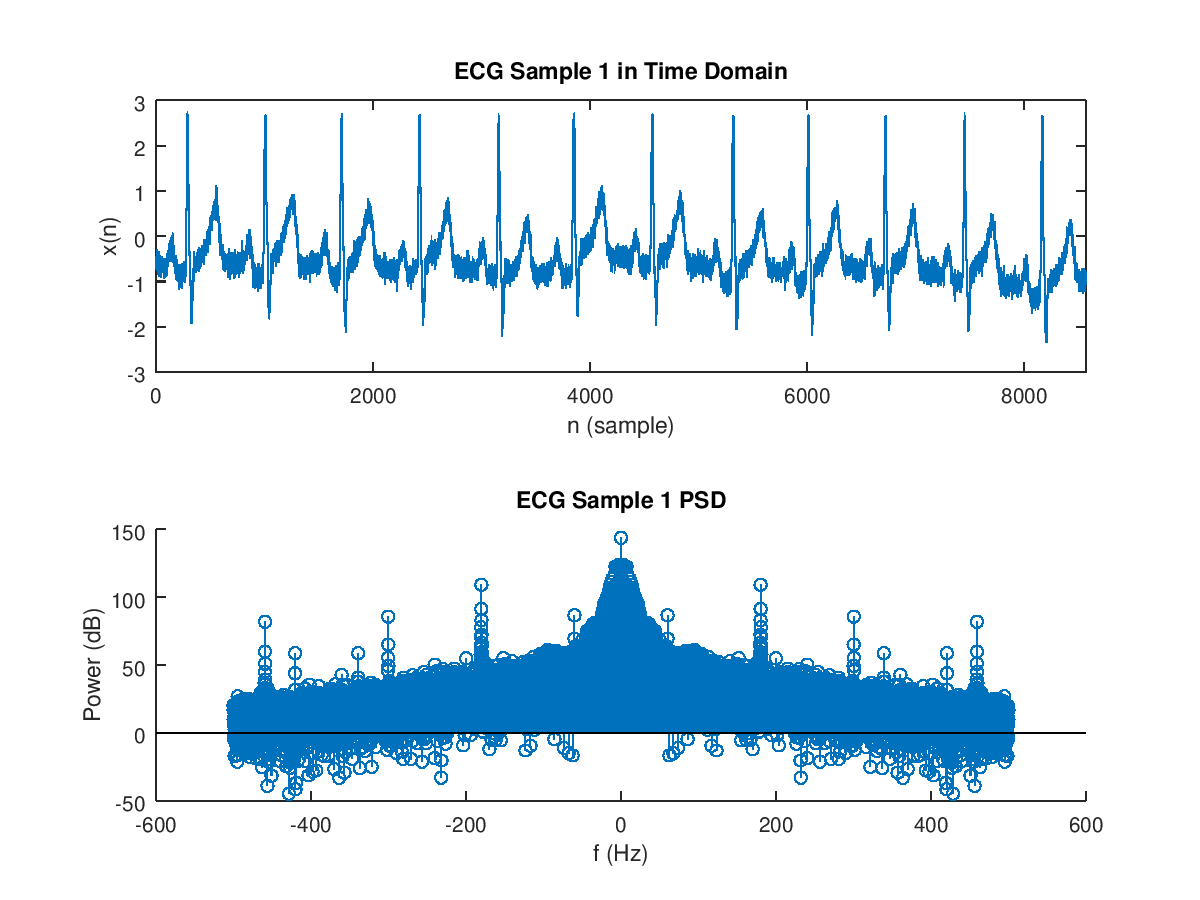
\includegraphics[scale=0.7]{figures/fig5-ecg1timeandpsd.png}}
\caption{Plot sampel ECG 1 dalam \textit{domain} waktu beserta PSD-nya}
\end{figure}

Sinyal sampel ECG 1 dalam \textit{domain} waktu berbentuk menyerupai bentuk \textit{template} dari sinyal ECG seperti pada gambar 1. Akan tetapi, bentuk sinyal sampel ECG 1 memiliki dua perbedaan utama dari bentuk \textit{template} sinyal ECG, yakni sinyal bergerak naik turun secara perlahan (mengalami pergeseran \textit{baseline}) yang menyebabkan letak puncak dan dasar sinyal berbeda antar siklus, serta terdapat fluktuasi sinyal yang terjadi secara cepat, atau selanjutnya disebut dengan \textit{jitter}, yang menyebabkan sinyal tidak 'halus'.

Karena sinyal sampel ECG 1 dicuplik dengan \textit{sample frequency} sebesar 1 kHz, akibat Teorema \textit{Sampling} Nyquist-Shannon, hasil FFT dari sinyal sampel ECG 1 memiliki rentang frekuensi antara -500 Hz hingga 500 Hz. Karena sinyal sampel ECG 1 bersifat \textit{real}, maka hasil FFT dari sinyal sampel ECG 1 bersifat genap. PSD dari sinyal merupakan kuadrat dari spektrum hasil FFT dari sinyal sampel ECG 1 sehingga PSD dari sinyal sampel ECG 1 pun bersifat genap dan memiliki rentang antara -500 Hz hingga 500 Hz.

Sinyal ECG yang bersih memiliki rentang frekuensi 0.5 hingga 20 Hz \cite{thakor84}. Pada PSD dari sampel ECG 1, tampak bahwa sinyal memiliki komponen frekuensi dari 0 hingga 500 Hz, dengan puncak-puncak pada frekuensi kelipatan 60 Hz yang merupakan frekuensi jala-jala yang digunakan, dan pada 0 Hz. Hal ini menunjukkan bahwa ketiga jenis derau yang dijelaskan pada bagian sebelumnya mencampuri sinyal sampel ECG 1, yakni derau berfrekuensi rendah, derau akibat interferensi jala-jala, serta derau berfrekuensi tinggi.

Derau berfrekuensi rendah pada sinyal sampel ECG 1 memiliki puncak pada frekuensi 0 Hz. Derau ini menyebabkan sinyal sampel ECG 1 mengalami pergeseran \textit{baseline} sehingga sinyal bergerak naik turun perlahan dalam \textit{domain} waktu.

Derau akibat interferensi jala-jala muncul pada frekuensi kelipatan 60 Hz. Akan tetapi, perhatikan bahwa derau hanya muncul pada kelipatan ganjil dari 60 Hz saja, yakni pada 180 Hz, 300 Hz, 420 Hz serta 840 Hz dan 960 Hz yang mengalami \textit{frequency folding} dan masing-masing muncul pada frekuensi 340 Hz dan 460 Hz. Hal ini menunjukkan bahwa sinyal jala-jala memiliki sifat \textit{half-wave symmetry} sehingga transformasi Fourier dari sinyal tersebut tidak memiliki harmonisa genap \cite{grady}.

Kemudian, meski tidak memiliki puncak, pada PSD tampak bahwa di atas rentang frekuensi sinyal ECG, terdapat komponen sinyal dengan daya sekitar 100 dB pada frekuensi tepat di atas 20 Hz, hingga 30 dB pada frekuensi 500 Hz. Hal ini menunjukkan bahwa terdapat derau yang tersebar pada frekuensi di atas rentang frekuensi sinyal ECG. Derau ini, bersama dengan derau akibat interferensi jala-jala menyebabkan \textit{jitter} pada sinyal sampel ECG 1 pada \textit{domain} waktu.

Kemudian, berikut adalah plot sinyal sampel ECG 2 dalam \textit{domain} waktu beserta dengan PSD-nya

\begin{figure}[H]
\centerline{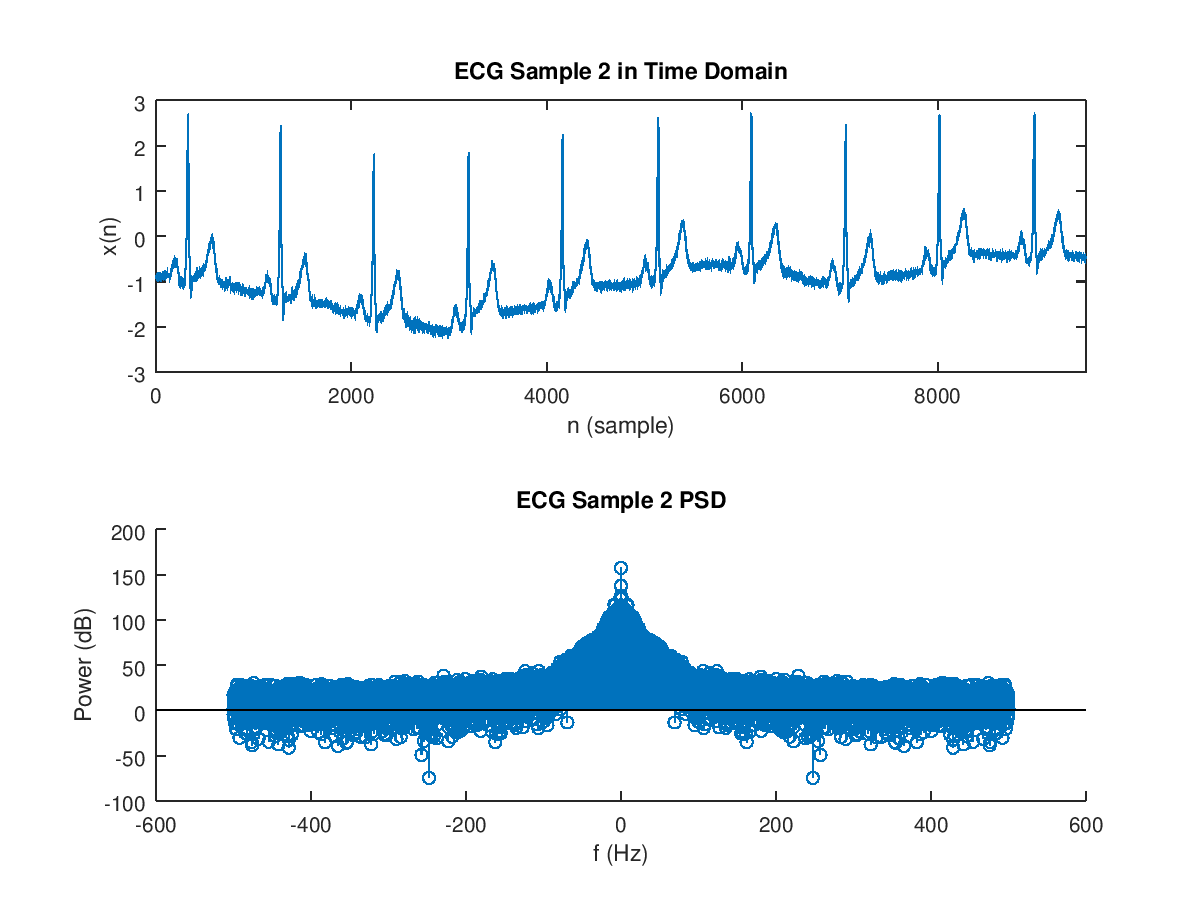
\includegraphics[scale=0.7]{figures/fig6-ecg2timeandpsd.png}}
\caption{Plot sampel ECG 2 dalam \textit{domain} waktu beserta PSD-nya}
\end{figure}

Hampir sama seperti sinyal sampel ECG 1, sinyal sampel ECG 2 pun memiliki bentuk umum menyerupai bentuk \textit{template} sinyal ECG. Hanya saja, sinyal sampel ECG 2 terlihat mengalami pergeseran \textit{baseline} yang lebih ekstrem dibandingkan sinyal sampel ECG 1. Selain itu, sinyal sampel ECG 2 juga mengalami \textit{jitter} yang menyebabkan sinyal sampel ECG 2 tidak tampak 'halus'.

PSD sinyal sampel ECG 2 menunjukkan bahwa meskipun sinyal memiliki derau yang tersebar pada seluruh rentang frekuensi, derau pada frekuensi rendah bersifat dominan, memiliki daya hingga 150 dB. Selain itu, derau akibat interferensi jala-jala tidak terlihat pada frekuensi kelipatan 60 Hz yang merupakan frekuensi jala-jala yang digunakan. Kemudian, seperti pada sinyal sampel ECG 1, sinyal sampel ECG 2 pun memliki derau berfrekuensi tinggi yang tersebar dari atas rentang frekuensi sinyal ECG hingga 500 Hz.

Derau berfrekuensi rendah yang memiliki amplitudo tinggi menyebabkan \textit{baseline} sinyal sampel ECG 2 naik turun secara ekstrem. Karena derau pada sinyal ini lebih kuat dibandingkan derau berfrekuensi rendah pada sinyal sampel ECG 1, sinyal sampel ECG 2 mengalami pergeseran \textit{baseline} yang lebih ekstrem dibandingkan sinyal sampel ECG 1. Derau ini memiliki puncak pada 0 Hz dan memiliki rentang frekuensi antara 0 Hz hingga sekitar 0.5 Hz.

Derau berfrekuensi tinggi pada sinyal ini tersebar dari atas rentang frekuensi ECG hingga frekuensi maksimum sinyal, 500 Hz. Seperti pada sinyal sampel ECG 1, derau berfrekuensi tinggi menyebabkan \textit{jitter} pada sinyal sampel ECG 2 dalam \textit{domain} waktu, meskipun \textit{jitter} yang terjadi lebih sedikit karena tidak ada atau lemahnya derau akibat interferensi jala-jala.

\subsection{Kode}

Berikut adalah kode \textit{Octave} yang digunakan pada topik 1. Secara garis besar, kode ini membaca kedua sinyal sampel ECG dari file *.dat, kemudian menghitung FFT dan PSD dari masing-masing sinyal, dan menampilkan kedua sinyal dalam \textit{domain} waktu dan PSD-nya dalam satuan dB. Kode ini tidak membutuhkan \textit{package} eksternal dan menggunakan \textit{built-in function} \textbf{fft}, \textbf{fftshift}, \textbf{abs}, dan \textbf{log10}.

\lstinputlisting[caption={Kode \textit{Octave} untuk Topik 1: Analisis Sinyal}]{octave_codes/topik_1.m}

\section{Topik II: Sistem Sebagai Filter}\label{topik-ii}

\subsection{Teori}

\subsubsection{Notch dan Comb Filter}

\textbf{Notch Filter} adalah sebuah filter yang memiliki satu atau lebih jurang, selanjutnya disebut dengan \textit{notch}, pada respons magnitudanya \cite{oppenheim}. Idealnya, \textit{notch filter} menghilangkan komponen frekuensi tertentu dari sinyal tanpa memengaruhi komponen frekuensi lain dari sinyal. \textit{Notch filter} berguna untuk keperluan yang membutuhkan kita untuk menghilangkan komponen frekuensi tertentu dari sinyal, seperti menghilangkan interferensi jala-jala beserta harmonisanya.

Untuk membuat \textit{notch} pada respons magnituda pada frekuensi $\omega_0$, kita hanya perlu menaruh sepasang \textit{zero} yang bersifat konjugat kompleks dengan satu sama lain pada lingkaran satuan pada sudut $\omega_0$ \cite{oppenheim}. Yakni pada

\begin{equation}
    z_{1,2} = e^{\pm j \omega_0}
\end{equation}

Dengan meletakkan \textit{pole} pada titik \textit{origin}, kita memperoleh \textit{notch filter} dengan \textit{finite impulse response} (FIR) yang memiliki fungsi transfer berikut

\begin{equation}
    H(z) = b_0 (1 - e^{j \omega_0} z^{-1}) (1 - e^{-j \omega_0} z^{-1})
    = b_0 (1 - 2 \cos{\omega_0 z^{-1}} + z^{-2})
\end{equation}

Meskipun \textit{notch filter} FIR memiliki respons fasa yang linear, \textit{notch filter} FIR memiliki \textit{bandwidth} yang cukup besar. Akibatnya, komponen frekuensi di sekitar \textit{notch} ikut teredam. Pada respons frekuensinya, tampak bahwa \textit{notch} yang terbentuk berbentuk landai.

\begin{figure}[H]
\centerline{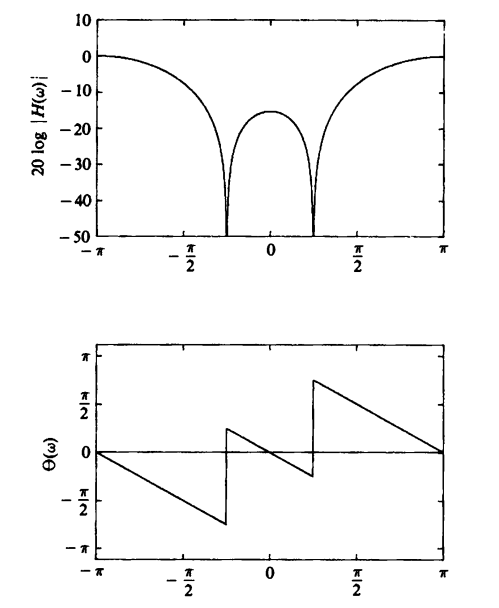
\includegraphics[scale=0.4]{figures/fig7-notchfreqresp.png}}
\caption{Respons frekuensi \textit{notch filter} FIR dengan \textit{notch} pada frekuensi $\omega = \frac{\pi}{4}$}
\end{figure}

Untuk mengurangi \textit{bandwidth} dari \textit{notch filter}, kita dapat meletakkan sepasang \textit{pole} yang bersifat konjugat kompleks terhadap satu sama lain di dalam lingkaran satuan dengan sudut yang sama dengan \textit{zero} yang telah diletakkan sebelumnya. Yakni pada

\begin{equation}
    z_{1,2} = r e^{\pm j \omega_0}
\end{equation}

Dengan $r$ merupakan bilangan real dengan nilai di antara 0 hingga 1 yang menunjukkan jarak \textit{pole} dari titik \textit{origin}. Dengan menambahkan \textit{pole}, \textit{bandwidth} dari \textit{notch filter} berkurang, akan tetapi penambahan \textit{pole} juga dapat menyebabkan sedikit \textit{ripple} pada \textit{passband} dari filter. Selain itu, respons fasa filter menjadi tidak linear dan filter memiliki \textit{infinite impulse response} (IIR). Setelah penambahan \textit{pole}, fungsi transfer dari \textit{notch filter} menjadi

\begin{equation}
    H(z) = b_0 \frac{1 - 2 \cos{\omega_0} z^{-1} + z^{-2}}{1 - 2r \cos{\omega_0} z^{-1} + r^2 z^{-2}}
\end{equation}

Sebagai contoh, berikut adalah plot respons frekuensi dari \textit{notch filter} dengan \textit{notch} pada $\frac{\pi}{4}$ setelah ditambahkan \textit{pole} pada $r = 0.85$ dan $r = 0.95$

\begin{figure}[H]
\centerline{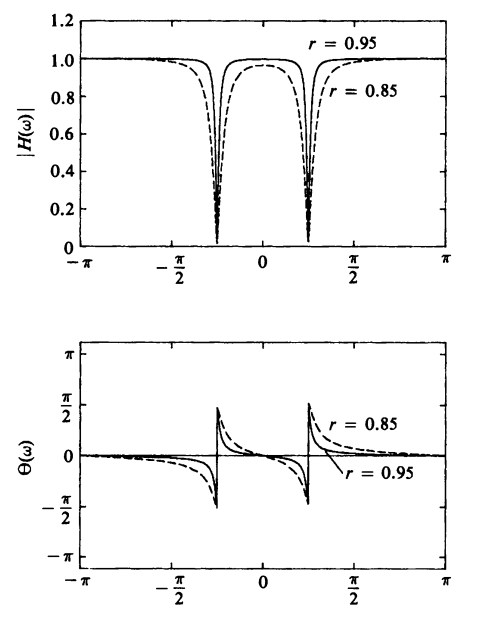
\includegraphics[scale=0.4]{figures/fig8-notchfreqrespwithpoles.png}}
\caption{Respons frekuensi \textit{notch filter} dengan \textit{notch} pada frekuensi $\omega = \frac{\pi}{4}$ dan \textit{pole} pada $r = 0.95$ dan $r = 0.85$}
\end{figure}

Untuk menghilangkan seluruh harmonisa dari derau akibat interferensi jala-jala, dapat digunakan \textbf{Comb Filter}. \textit{Comb filter} dapat dibuat dengan merangkai beberapa \textit{notch filter} pada frekuensi yang berkelipatan secara kaskade. Dengan demikian, diperoleh bentuk respons frekuensi yang menyerupai sebuah sisir, maka dari itu filter ini disebut \textit{comb filter}.

\subsubsection{Bandpass Filter}

\textbf{Bandpass Filter} adalah jenis filter selektif frekuensi yang meloloskan sinyal dengan rentang frekuensi tertentu dan meredam sinyal di luar rentang tersebut. Berikut adalah respons magnituda dari \textit{bandpass filter} ideal

\begin{figure}[H]
\centerline{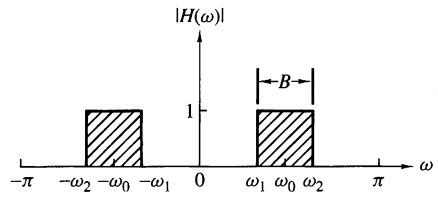
\includegraphics[scale=0.4]{figures/fig9-bpfideal.png}}
\caption{Respons frekuensi \textit{bandpass filter} ideal}
\label{bpfideal}
\end{figure}

\textit{Bandpass filter} dapat diimplementasikan dengan beberapa cara. Salah satunya adalah dengan merangkai \textit{lowpass filter} yang memiliki frekuensi \textit{cutoff} tinggi dengan \textit{highpass filter} yang memiliki frekuensi \textit{cutoff} rendah secara kaskade. Dengan demikian, akan diperoleh respons frekuensi gabungan dari kedua filter tersebut, yang menghasilkan respons frekuensi seperti pada Gambar \ref{bpfideal}.

Terdapat beberapa pendekatan standar untuk merancang \textit{bandpass filter} digital. Beberapa di antaranya adalah dengan merancang \textit{bandpass filter} analog terlebih dahulu kemudian melakukan transformasi filter yang telah dirancang ke \textit{domain} digital, dan dengan melakukan teknik \textit{windowing}. Pada laporan ini, hanya akan dibahas pendekatan perancangan \textit{bandpass filter} dengan merancang filter analog terlebih dahulu kemudian melakukan transformasi ke \textit{domain} digital.

Pendekatan perancangan \textit{bandpass filter} digital dengan merancang filter analog terlebih dahulu dilakukan karena ilmu perancangan filter analog yang lebih \textit{well-established} dibandingkan dengan ilmu perancangan filter digital.
Salah satu \textit{template} filter yang umum adalah filter Butterworth dan Chebyshev. Filter Butterworth memiliki karakteristik respons frekuensi tanpa \textit{ripple} pada \textit{passband} dan \textit{stopband}-nya dengan \textit{trade-off} \textit{transition band} yang landai dan panjang. Di sisi lain, filter Chebyshev memiliki \textit{transition band} yang pendek namun dengan \textit{ripple} pada \textit{passband} dan \textit{stopband}-nya.

\begin{figure}[H]
\centerline{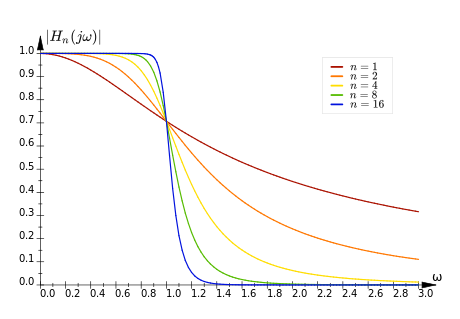
\includegraphics[scale=0.5]{figures/fig10-butterlpfresponse.png}}
\caption{Respons frekuensi filter \textit{lowpass} Butterworth ternormalisasi}
\end{figure}

Perancangan filter Butterworth pada umumnya dimulai dengan merancang \textit{lowpass filter} yang ternormalisasi, yakni memiliki frekuensi \textit{cutoff} pada $\omega_c = 1$ Hz kemudian dilakukan transformasi pada filter tersebut sehingga diperoleh filter dengan jenis dan frekuensi \textit{cutoff} yang diinginkan. 

\textit{Lowpass filter} analog Butterworth berorde $n$ dan frekuensi \textit{cutoff} $\omega_c$ didefinisikan memiliki fungsi transfer berikut
    
\begin{equation}
    |H_n(s)| = \frac{1}{\sqrt{1 + (\frac{s}{\omega_c})^{2n}}} = \frac{1}{B_n (\frac{s}{\omega_c})}
\end{equation}

Sedangkan \textit{highpass filter} analog Butterworth berorde $n$ dan frekuensi \textit{cutoff} $\omega_c$ didefinisikan memiliki fungsi transfer berikut

\begin{equation}
    |H_n(s)| = \frac{1}{\sqrt{1 + (\frac{s}{\omega_c})^{-2n}}} = \frac{s^n}{\omega_c^n B_n (\frac{s}{\omega_c})}
\end{equation}

Dengan $B_n$ merupakan polinom Butterworth yang didefinisikan sebagai

\begin{equation}
    B_n(s) = 
    \left\{
    	\begin{array}{ll}
    		\prod_{k = 0}^{\frac{n}{2} -1} (s^2 - 2 \cos{2 \pi \frac{2k + n + 1}{4n} s + 1})  & \mbox{} n \text{ genap} \\
    		(s + 1) \prod_{k = 0}^{\frac{n-1}{2} -1} (s^2 - 2 \cos{2 \pi \frac{2k + n + 1}{4n} s + 1}) & \mbox{} n \text{ ganjil}
    	\end{array}
    \right.
\end{equation}

Setelah merancang \textit{lowpass filter} dan \textit{highpass filter} dengan frekuensi \textit{cutoff} yang sesuai, fungsi transfer dari kedua filter dikalikan untuk memperoleh fungsi transfer \textit{bandpass filter} Butterworth analog. Setelah itu, dapat dilakukan pendekatan digital atas \textit{bandpass filter} analog yang telah dirancang, salah satunya adalah dengan transformasi Bilinear juga dikenal sebagai transformasi Tustin, yakni dengan mensubstitusikan

\begin{equation}
    s \leftarrow \frac{2 (z -1)}{ T (z + 1)}
\end{equation}

Dengan $T$ merupakan \textit{sample time} dari sistem. Setelah dilakukan transformasi Tustin, diperoleh fungsi transfer filter \textit{lowpass} Butterworth sebagai berikut

\begin{equation}
    H_n(z) = \frac{Z_n(z)}{P_n(z)}
\end{equation}

Dengan $Z_n(z)$ dan $P_n(z)$ masing-masing merupakan polinom \textit{zero} dan \textit{pole} dari filter yang didefinisikan sebagai

\begin{equation}
    Z_n(z) = 
    \left\{
    	\begin{array}{ll}
    		\prod_{k = 0}^{\frac{n}{2} -1} (1 + 2 z^{-1} + z^{-2})  & \mbox{} n \text{ genap} \\
    		(1 - z^{-1})\prod_{k = 0}^{\frac{n - 1}{2} -1} (1 + 2 z^{-1} + z^{-2}) & \mbox{} n \text{ ganjil}
    	\end{array}
    \right.
\end{equation}

\begin{equation}
    P_n(z) = 
    \left\{
    	\begin{array}{ll}
    		\prod_{k = 0}^{\frac{n}{2} -1} ((\gamma^2 - \alpha \gamma + 1) + (-2 \gamma^2 + 2) z^{-1} + (\gamma^2 + \alpha \gamma + 1) z^{-2})  & \mbox{} n \text{ genap} \\
    		((\gamma + 1) + (1 - \gamma) z^{-1})\prod_{k = 0}^{\frac{n - 1}{2} -1} ((\gamma^2 - \alpha \gamma + 1) + (-2 \gamma^2 + 2) z^{-1} + (\gamma^2 + \alpha \gamma + 1) z^{-2}) & \mbox{} n \text{ ganjil}
    	\end{array}
    \right.
\end{equation}

Dengan $\gamma$ dan $\alpha$ suatu konstanta yang didefinisikan sebagai

\begin{equation}
    \gamma = \cot{\frac{\omega_c \pi}{F_s}}
\end{equation}

\begin{equation}
    \alpha = 2 \cos{2 \pi \frac{2 k + n + 1}{4 n}}
\end{equation}

Dengan $F_s$ merupakan \textit{sample frequency} dari sistem. Sedangkan untuk filter \textit{highpass} Butterworth, $Z_n(z)$ didefinisikan sebagai

\begin{equation}
    Z_n(z) = \prod_{k = 1}^{n} (\gamma - \gamma z^{-1})
\end{equation}

\subsection{Perancangan Filter}

\subsubsection{Pengolahan Sinyal}

Berdasarkan pembahasan pada topik \ref{topik-i}, diperoleh bahwa pada kedua sinyal sampel ECG yang diberikan terdapat tiga jenis derau: derau berfrekuensi rendah, derau akibat interferensi jala-jala, dan derau berfrekuensi tinggi. Karena itu, diperlukan filter untuk menghilangkan ketiga jenis derau tersebut. Untuk derau berfrekuensi rendah dan tinggi akan dirancang sebuah \textit{bandpass filter} dan untuk derau akibat interferensi jala-jala akan dirancang sebuah \textit{comb filter}.

\subsubsection{Perancangan \textit{Bandpass Filter}}
Sinyal ECG memiliki rentang frekuensi antara 0.5 Hz hingga 20 Hz. Karenanya, \textit{bandpass filter} yang dirancang memiliki frekuensi \textit{cutoff} pada $\omega_1 = 0.5$ Hz dan $\omega_2 = 20$ Hz. Dengan mengatur frekuensi \textit{cutoff} pada nilai tersebut, \textit{bandpass filter} akan mampu menghilangkan derau berfrekuensi DC dan rendah, derau berfrekuensi tinggi, serta membantu meredam derau akibat interferensi jala-jala.

Sinyal ECG memiliki informasi dalam \textit{domain} waktu. Karena itu, penting bagi filter untuk tidak memiliki \textit{ripple} pada respons frekuensinya agar perubahan bentuk sinyal dalam \textit{domain} waktu dapat diminimalkan. Untuk itu, dipilihlah filter Butterworth karena respons frekuensinya yang \textit{maximally flat} atau dengan kata lain tidak memiliki \textit{ripple}.

Setelah memilih orde filter 4 untuk \textit{lowpass} dan \textit{highpass filter}, dengan frekuensi \textit{cutoff} di atas diperoleh \textit{pole-zero plot} dari \textit{bandpass filter} sebagai berikut

\begin{figure}[H]
\begin{subfigure}
    \centering
    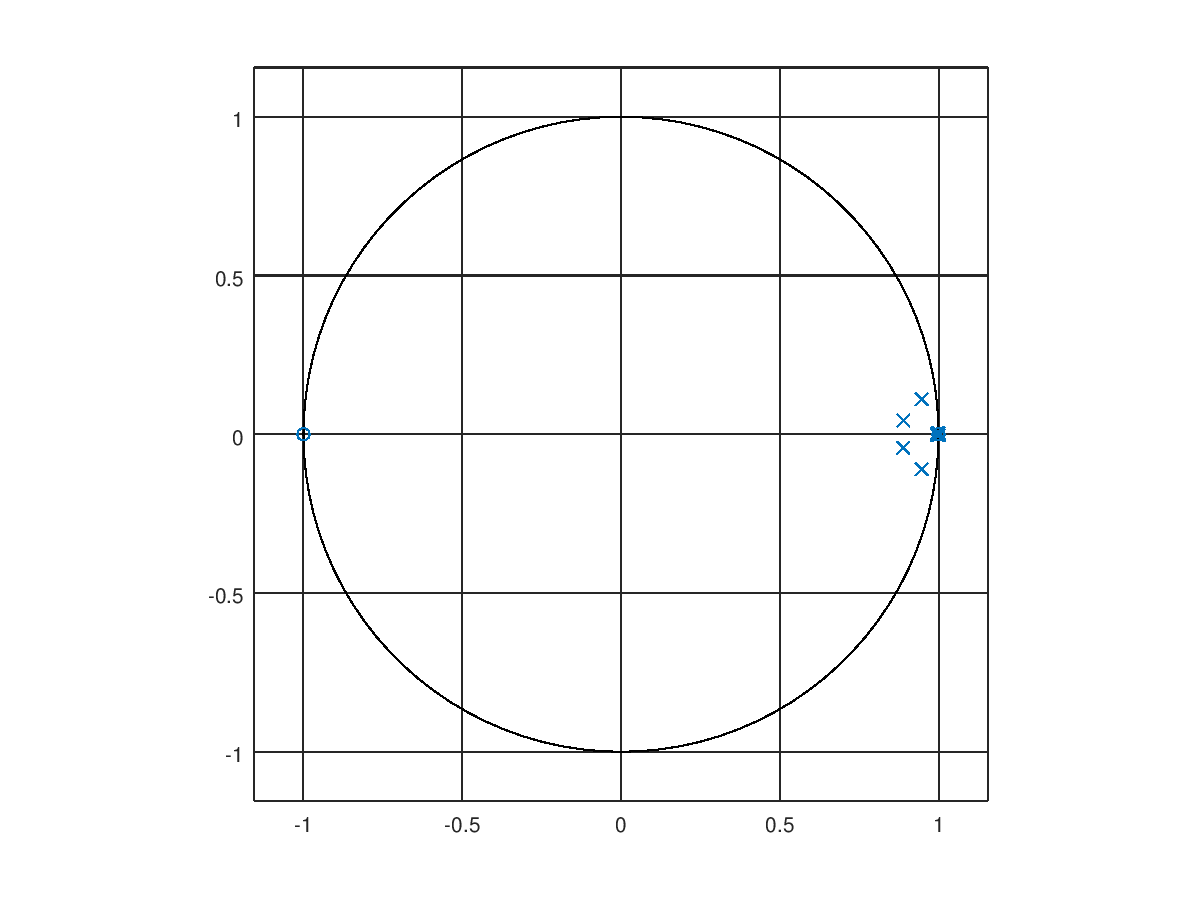
\includegraphics[scale=0.5]{figures/fig11-bpfpzp.png}
\end{subfigure}
\begin{subfigure}
    \centering
    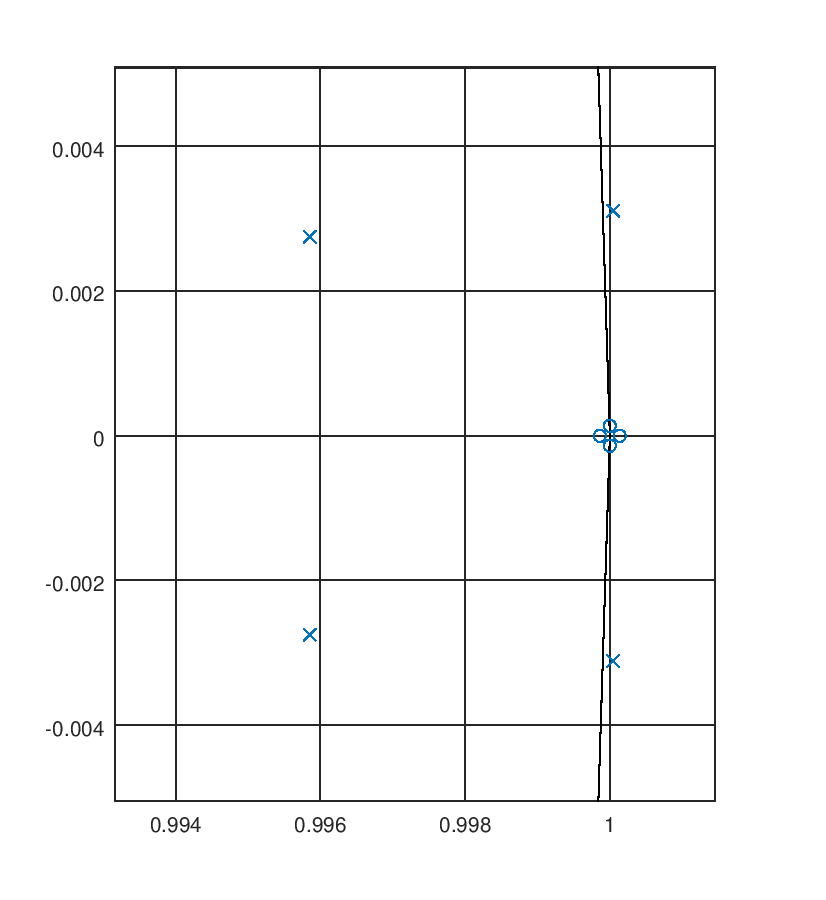
\includegraphics[scale=0.25]{figures/fig12-bpfpzp2.png}
\end{subfigure}
\caption{\textit{Pole-zero plot} dari \textit{bandpass filter} Butterworth orde 4 dengan $\omega_1 = 0.5$ Hz dan $\omega_2 = 20$ Hz}
\end{figure}

Filter yang diperoleh memiliki delapan buah \textit{pole} di sekitar $\omega = 0$ dan delapan buah \textit{zero} dengan empat buah \textit{zero} di sekitar $\omega = 0$ dan empat buah \textit{zero} di $\omega = \pi$.

Filter ini memiliki respons frekuensi sebagai berikut:

\begin{figure}[H]
\centerline{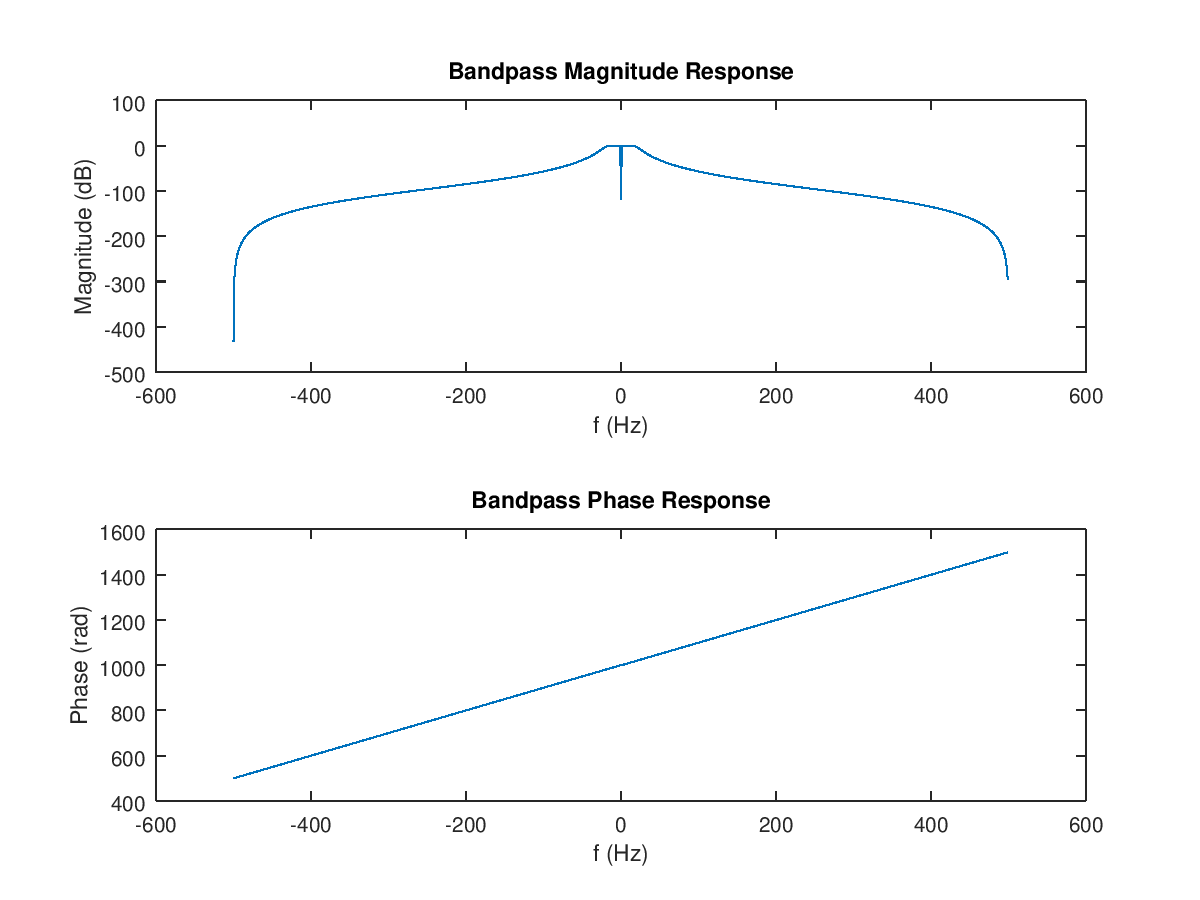
\includegraphics[scale=0.7]{figures/fig13-bpffreqresp.png}}
\centerline{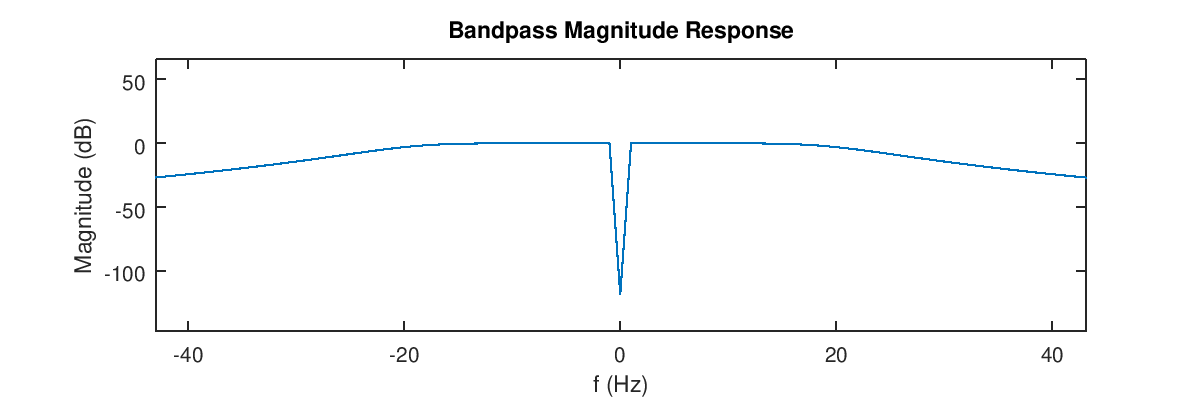
\includegraphics[scale=0.335]{figures/fig14-bpfmagresp.png}}
\caption{Respons frekuensi \textit{bandpass filter} Butterworth orde 4 dengan $\omega_1 = 0.5$ Hz dan $\omega_2 = 20$ Hz}
\label{bpffreqresp}
\end{figure}

Dari plot respons frekuensi \textit{bandpass filter}, terlihat bahwa \textit{bandpass filter} berperilaku seperti seharusnya dan memang memiliki frekuensi \textit{cutoff} pada $\omega_1 = 0.5$ Hz dan $\omega_2 = 20$ Hz. \textit{bandpass filter} melemahkan dengan tajam komponen sinyal berfrekuensi di bawah 0.5 Hz dan melemahkan secara relatif tidak terlalu tajam komponen sinyal berfrekuensi di atas 20 Hz. 

\begin{figure}[H]
\centerline{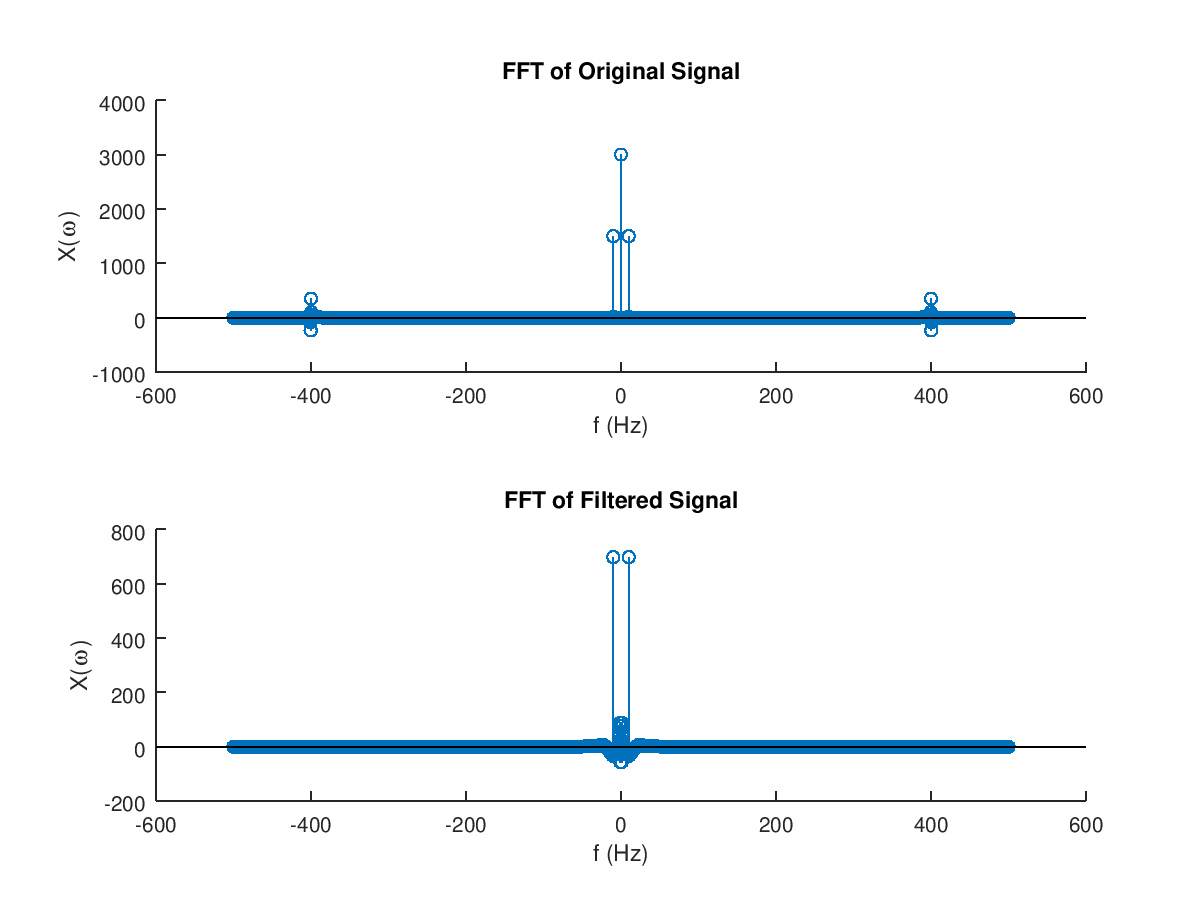
\includegraphics[scale=0.55]{figures/fig16-bpfcosspectrum.png}}
\centerline{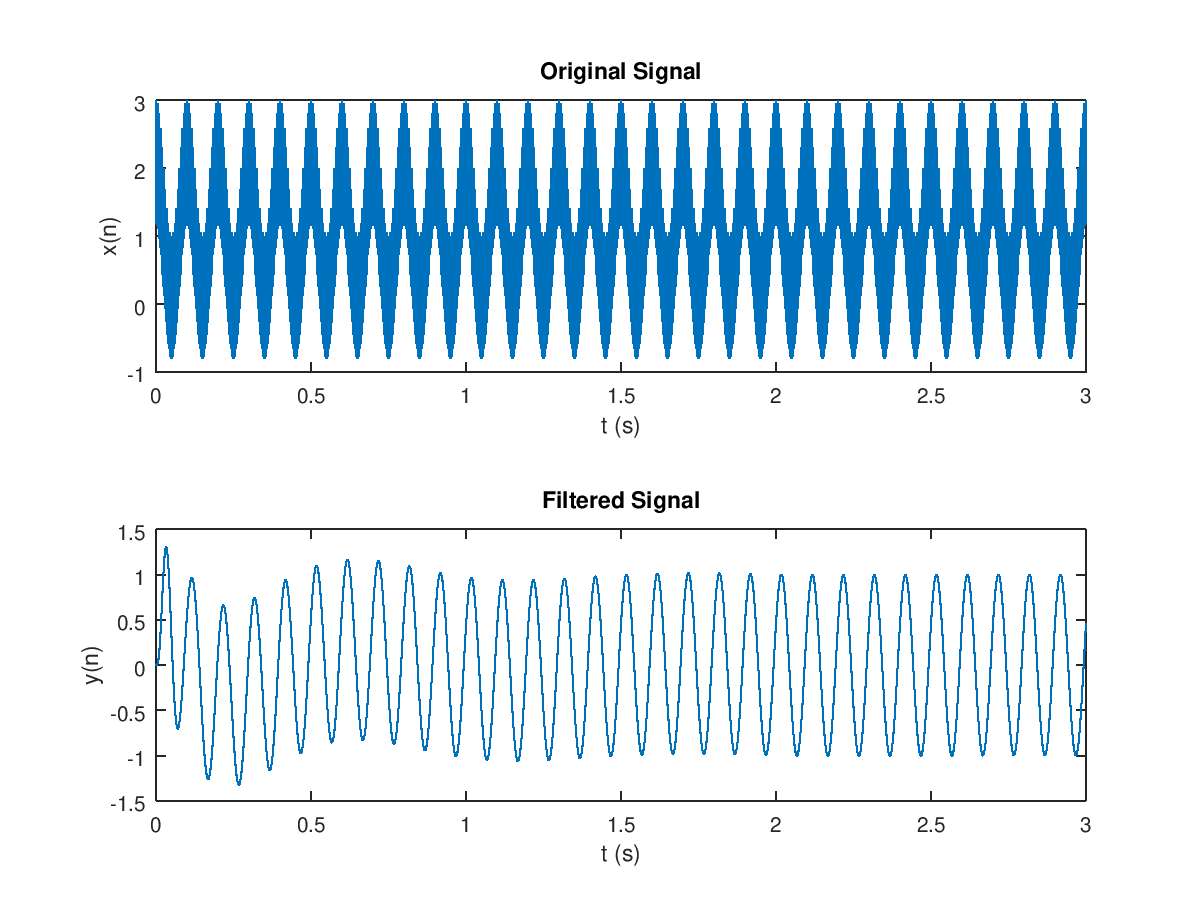
\includegraphics[scale=0.55]{figures/fig15-bpfcostrial.png}}
\caption{Hasil uji coba filter \textit{bandpass} pada sinyal cosinus gabungan frekuensi 0.01 Hz, 10 Hz, dan 400 Hz dan FFT-nya}
\label{bpfcosresp}
\end{figure}

Untuk menguji coba filter ini, digunakan sebuah sinyal input yang terdiri atas tiga buah sinyal cosinus yang digabungkan, masing-masing berfrekuensi 0.01 Hz, 10 Hz, dan 400 Hz. Seperti yang terlihat pada hasil FFT dari sinyal, filter berhasil meredam komponen cosinus dengan frekuensi 0.01 Hz dan 400 Hz, menyisakan komponen cosinus yang memiliki frekuensi pada \textit{passband} dari filter, yakni pada 10 Hz. 

Pada awal sinyal hasil filter pada \textit{domain} waktu, tampak sedikit fluktuasi \textit{baseline} dari sinyal. Hal ini dikarenakan proses \textit{filtering} yang dilakukan mengasumsikan kondisi rileks, sehingga butuh waktu agar komponen cosinus berfrekuensi rendah hilang. Selain itu, juga tampak bahwa \textit{jitter} pada sinyal, yang disebabkan oleh komponen cosinus berfrekuensi tinggi, hilang pada sinyal hasil \textit{filtering}. Setelah beberapa saat, sinyal hasil \textit{filtering} berbentuk cosinus dengan frekuensi 10 Hz murni, seperti yang diharapkan.

\subsubsection{Perancangan \textit{Comb Filter}}

Berdasarkan hasil analisis sinyal pada topik \ref{topik-i}, diperoleh bahwa sinyal sampel ECG yang diberikan memiliki derau akibat interferensi jala-jala pada frekuensi 60 Hz beserta harmonisanya. Untuk menghilangkan derau tersebut, dirancang sebuah \textit{notch filter} untuk setiap frekuensi harmonisa dari frekuensi jala-jala. Karena itu, diperlukan notch filter sejumlah

\begin{equation}
    n = \floor{\frac{F_s}{f_{jala-jala}}} = \floor{\frac{1000}{60}} = 16
\end{equation}

Sehingga akan diperoleh \textit{comb filter} dengan 32 buah \textit{notch}, 32 buah \textit{pole} dan 32 buah \textit{zero} pada sudut kelipatan

\begin{equation}
    \omega = \frac{f_{jala-jala}}{F_s} = \frac{60}{1000} = 0.06 \text{ /siklus} = 0.3769 \text{ rad/s}
\end{equation}

Dengan mengambil jarak \textit{pole} dari origin sebesar $r = 0.995$, diperoleh \textit{pole-zero plot} berikut

\begin{figure}[H]
\centerline{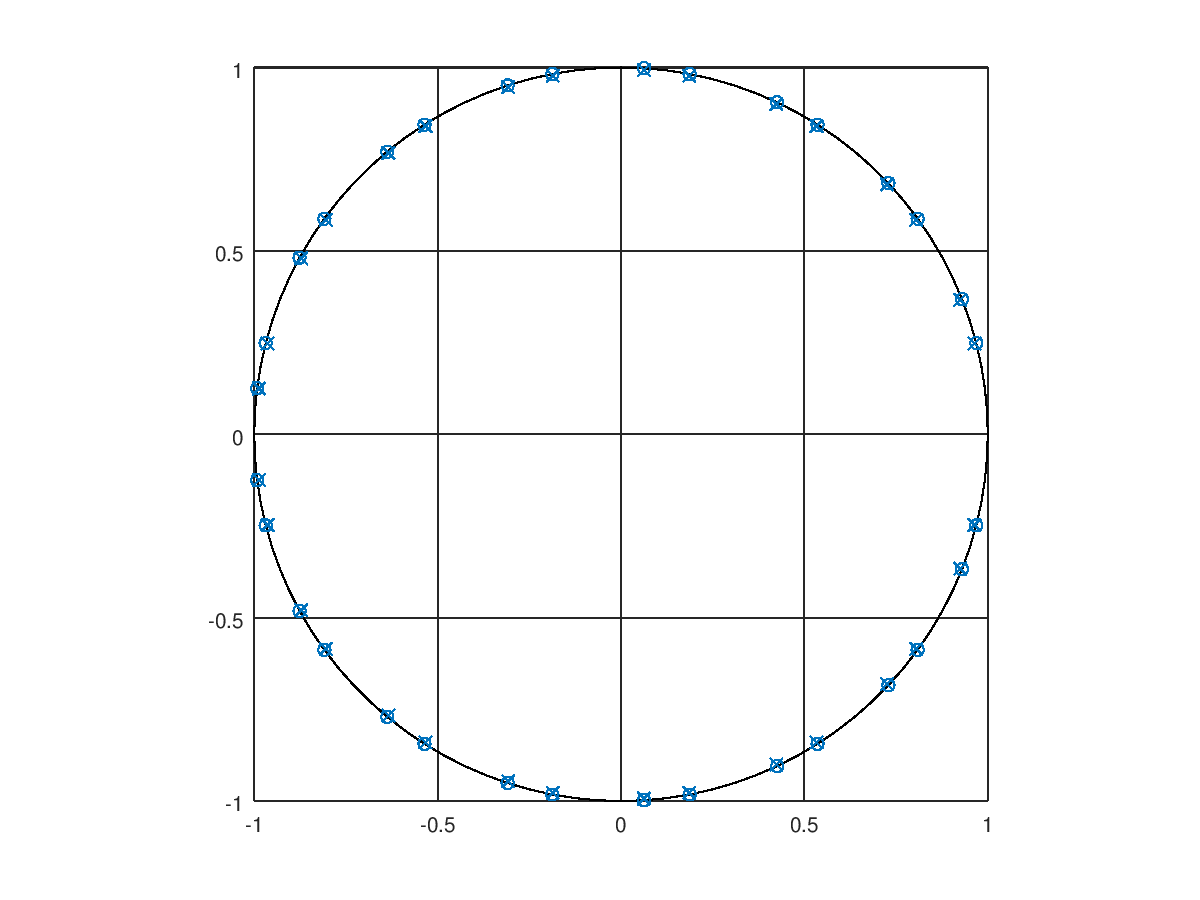
\includegraphics[scale=0.5]{figures/fig17-combpzp.png}}
\caption{\textit{Pole-zero plot} dari \textit{comb filter}}
\label{bpffreqresp}
\end{figure}

Filter ini memiliki respons frekuensi sebagai berikut

\begin{figure}[H]
\centerline{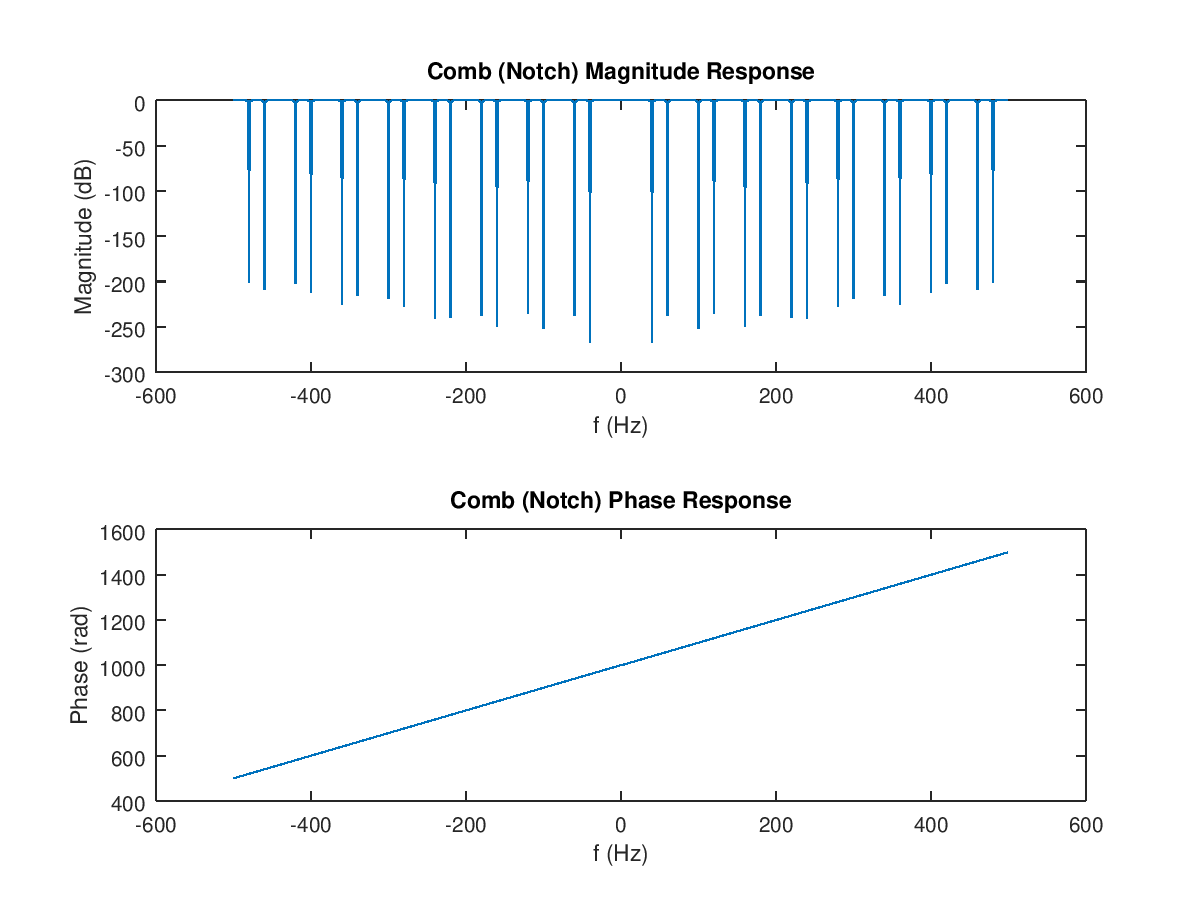
\includegraphics[scale=0.7]{figures/fig18-combfreqresp.png}}
\caption{Respons frekuensi dari \textit{comb filter}}
\label{combfreqresp}
\end{figure}

Pada respons magnituda dari filter, terdapat 32 buah \textit{notch} pada frekuensi 60 Hz beserta dengan kelipatannya. \textit{Notch} pada frekuensi lebih dari setengah \textit{sample frequency}, 500 Hz, mengalami \textit{frequency folding} ke frekuensi di bawah 500 Hz.

Meskipun merupakan filter IIR, respons fasa dari \textit{comb filter} yang diperoleh bersifat linear. Sifat ini penting karena sinyal ECG memiliki informasi dalam \textit{domain} waktu. Respons fasa yang linear menggeser tiap komponen frekuensi dari sinyal ECG sejauh suatu besaran waktu yang sama besar di \textit{domain} waktu sehingga bentuk dari sinyal akan terjaga.

Untuk menguji filter yang dirancang, diberikan sinyal \textit{input} yang terdiri atas penjumlahan tiga buah sinyal cosinus berfrekuensi masing-masing 10 Hz, 60 Hz, dan 120 Hz. Pemilihan frekuensi komponen sinyal cosinus ini dikarenakan frekuensi 10 Hz termasuk dalam rentang frekuensi \textit{passband} dari filter, sedangkan frekuensi 60 Hz dan 120 Hz merupakan frekuensi salah satu \textit{notch} dari filter.

Berikut adalah hasil pengujian \textit{comb filter} dengan sinyal \textit{input} tersebut

\begin{figure}[H]
\centerline{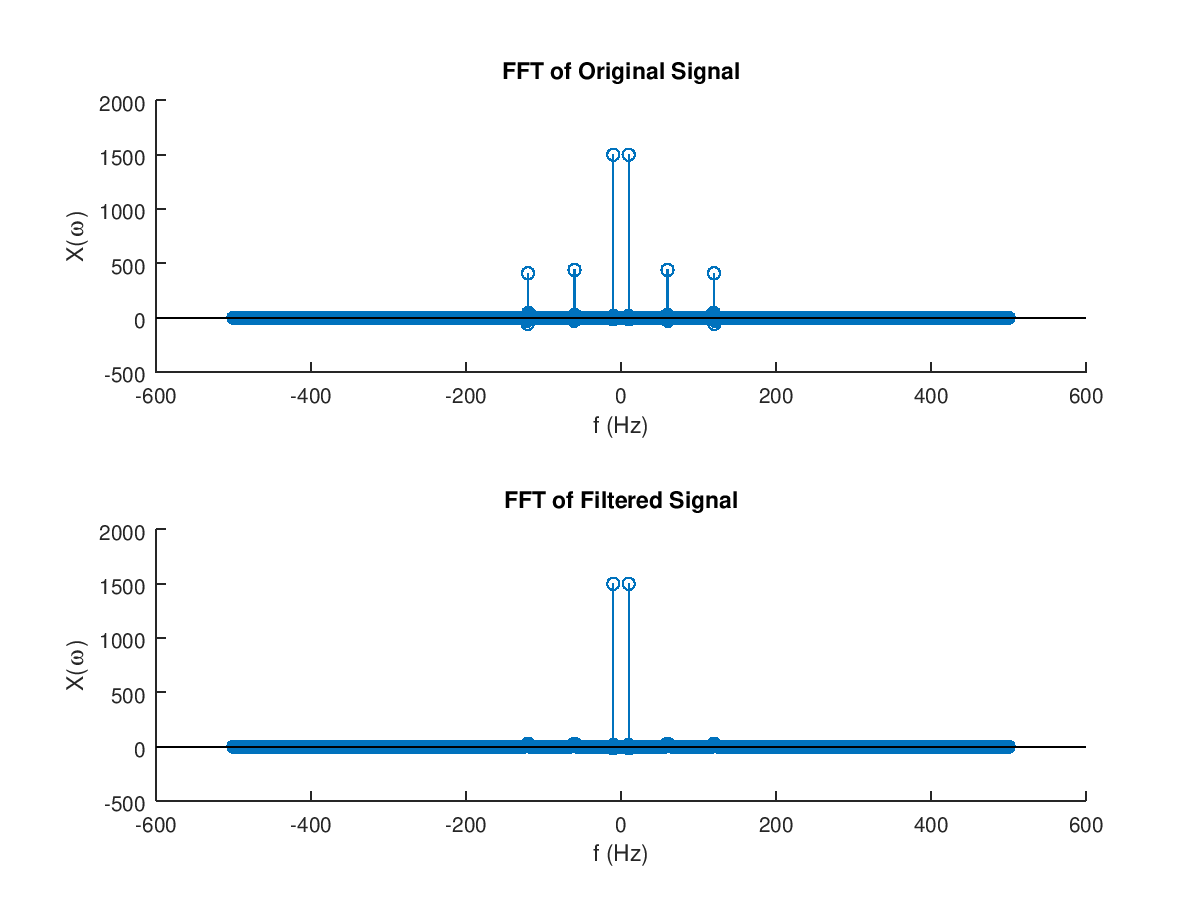
\includegraphics[scale=0.55]{figures/fig20-combcosspectrum.png}}
\centerline{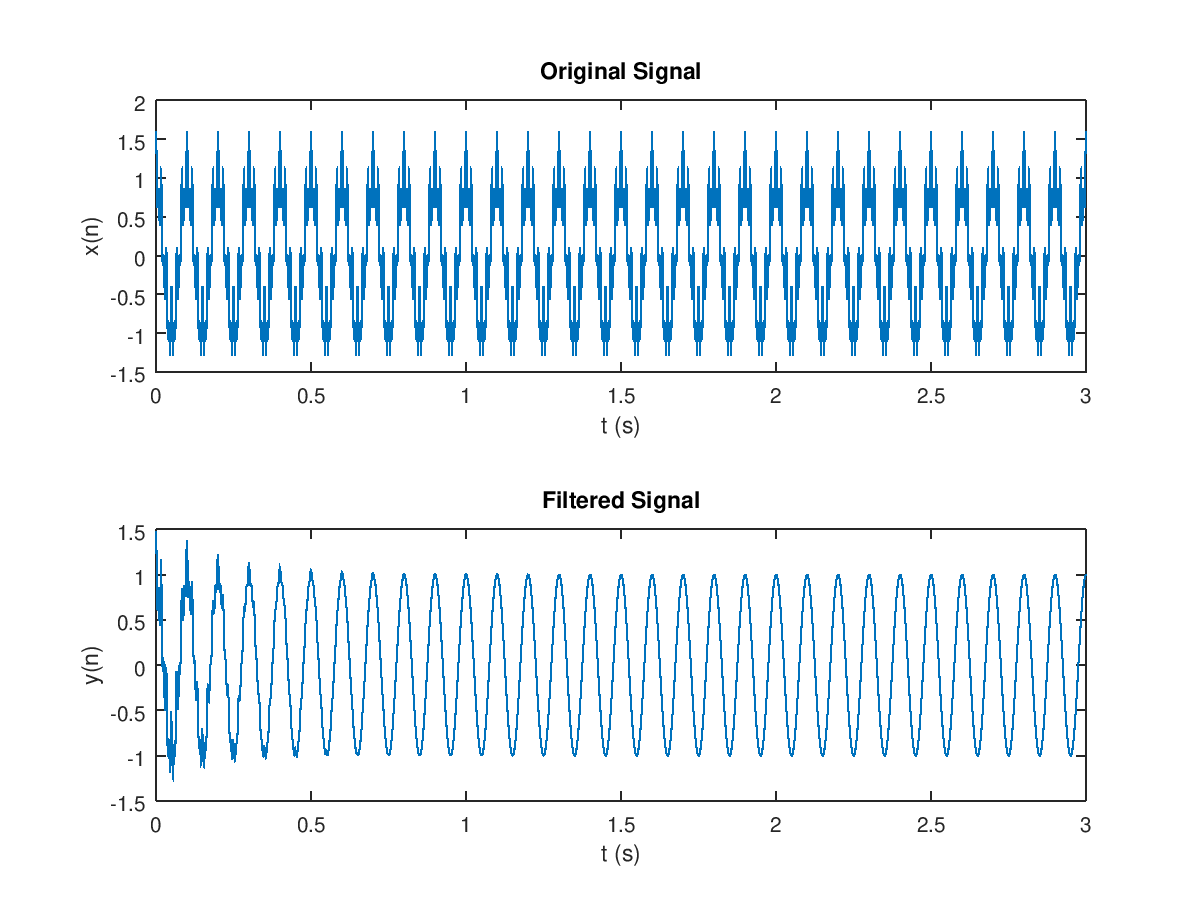
\includegraphics[scale=0.55]{figures/fig19-combcostrial.png}}
\caption{Hasil uji coba \textit{comb filter} pada sinyal cosinus gabungan frekuensi 10 Hz, 60 Hz, dan 120 Hz dan FFT-nya}
\label{combcosresp}
\end{figure}

Hasil FFT dari sinyal \textit{input} dan sinyal yang telah difilter menunjukkan bahwa \textit{notch} pada frekuensi 60 Hz dan 120 Hz bekerja dengan efektif untuk menghilangkan komponen frekuensi tersebut dari sinyal gabungan. Kemudian, terlihat bahwa komponen frekuensi 10 Hz dari sinyal gabungan tidak mengalami perubahan magnituda. Hal ini menunjukkan bahwa \textit{comb filter} tidak meredam komponen frekuensi pada rentang frekuensi \textit{passband}-nya.

Pada sinyal \textit{domain} waktu, tampak bahwa seiring berjalannya waktu, sinyal berbentuk \textit{cosinus} murni berfrekuensi 10 Hz. Hal ini menunjukkan bahwa \textit{comb filter} bekerja seperti seharusnya. Namun, pada awalnya, sinyal hasil \textit{filtering} terlihat mengandung derau. Sama seperti pada pengujian \textit{bandpass filter}, hal ini dikarenakan proses \textit{filtering} mengasumsikan kondisi awal rileks, sedangkan kondisi awal sebenarnya tidak demikian.

\subsection{Hasil dan Pembahasan}

Diberikan dua sinyal sampel ECG yang dianalisis pada topik \ref{topik-i}. Kedua sinyal sampel ECG tersebut akan difilter dengan kedua filter yang telah dirancang pada bagian sebelumnya yang dirangkai secara kaskade. Berikut adalah PSD sinyal mentah dan sinyal hasil proses \textit{filtering} yang dilakukan pada sinyal sampel ECG 1

\begin{figure}[H]
\centerline{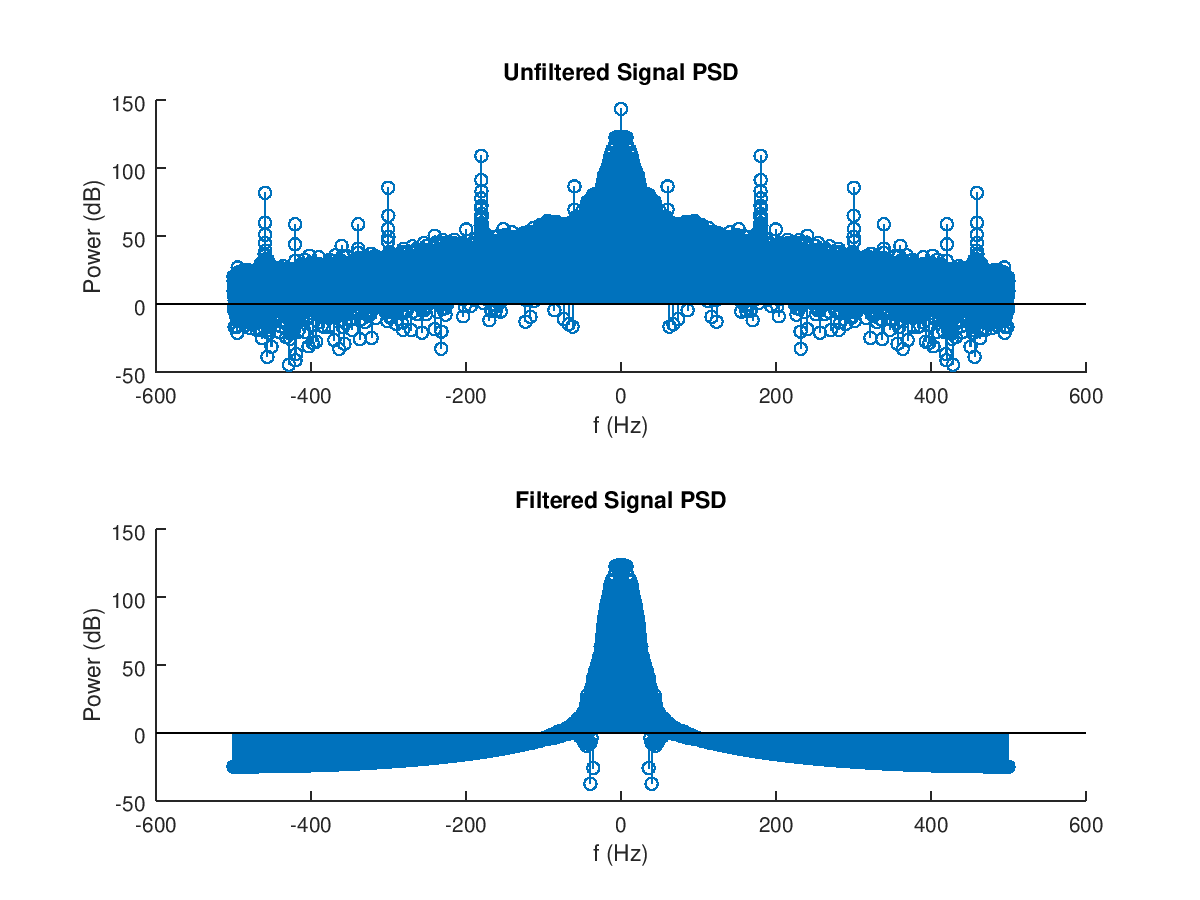
\includegraphics[scale=0.55]{figures/fig22-ecg1filteredpsd.png}}
\caption{PSD hasil proses \textit{filtering} terhadap sinyal sampel ECG 1}
\label{ecg1filteredpsd}
\end{figure}

Sebelum dilakukan proses \textit{filtering}, PSD sinyal memiliki banyak lonjakan daya pada frekuensi jala-jala dan kelipatannya serta pada frekuensi rendah. Selain itu, daya dari sinyal tersebar pada seluruh rentang frekuensi yang ada. 

Setelah mengalami proses \textit{filtering}, lonjakan daya pada frekuensi jala-jala dan kelipatannya hilang. Hal ini dikarenakan penggunaan \textit{comb filter} yang meredam komponen frekuensi jala-jala dan kelipatannya dari sinyal dan sesedikit mungkin memengaruhi daerah di sekitarnya. Kemudian, peredaman komponen frekuensi jala-jala dan kelipatannya turut dibantu oleh penggunaan \textit{bandpass filter} yang memiliki frekuensi \textit{cutoff} \textit{lowpass} pada frekuensi 20 Hz, lebih rendah dibandingkan harmonisa pertama dari frekuensi jala-jala yakni 60 Hz sehingga seluruh harmonisa dari frekuensi jala-jala turut teredam. Hasil dari peredaman ini tampak pada PSD sinyal yang telah melewati proses \textit{filtering} yang halus dan tidak memiliki lonjakan daya pada frekuensi tertentu.

Selain itu, setelah mengalami proses \textit{filtering}, lonjakan daya pada frekuensi rendah dan frekuensi DC dan sebaran daya pada frekuensi tinggi turut hilang.  Hal ini dikarenakan penggunaan \textit{bandpass filter} yang memblok komponen sinyal berfrekuensi di bawah 0.5 Hz dan di atas 20 Hz. Akibatnya, derau frekuensi rendah hilang dan derau pada frekuensi tinggi diredam sehingga diperoleh PSD sinyal yang terkonsentrasi pada rentang frekuensi sinyal ECG, yakni dari 0.5 Hz hingga 20 Hz seperti yang diharapkan.

\begin{figure}[H]
\centerline{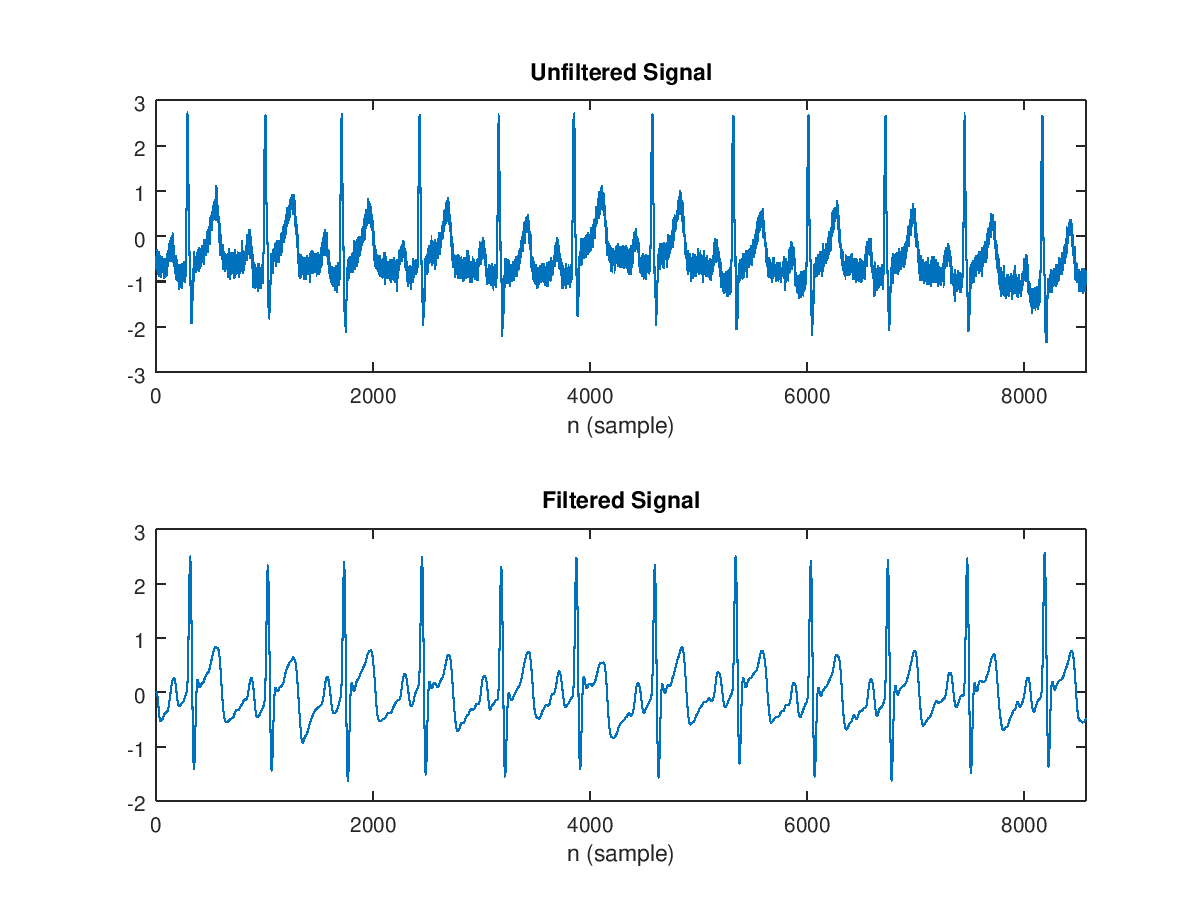
\includegraphics[scale=0.55]{figures/fig21-ecg1filteredtime.png}}
\caption{Hasil proses \textit{filtering} terhadap sinyal sampel ECG 1 dalam \textit{domain} waktu}
\label{ecg1filteredtime}
\end{figure}

Sinyal dalam \textit{domain} waktu sebelum proses \textit{filtering} tampak memiliki sedikit pergeseran \textit{baseline} dan mengalami banyak \textit{jitter}. Setelah mengalami proses \textit{filtering}, diperoleh sinyal dengan \textit{baseline} yang relatif lebih sedikit. Selain itu, sinyal hasil proses \textit{filtering} mengalami \textit{jitter} yang jauh lebih sedikit atau bahkan tidak ada, dan diperoleh sinyal yang sangat halus sesuai dengan \textit{template} sinyal ECG.

Kemudian, berikut adalah PSD sinyal mentah dan sinyal hasil proses \textit{filtering} yang dilakukan pada sinyal sampel ECG 2

\begin{figure}[H]
\centerline{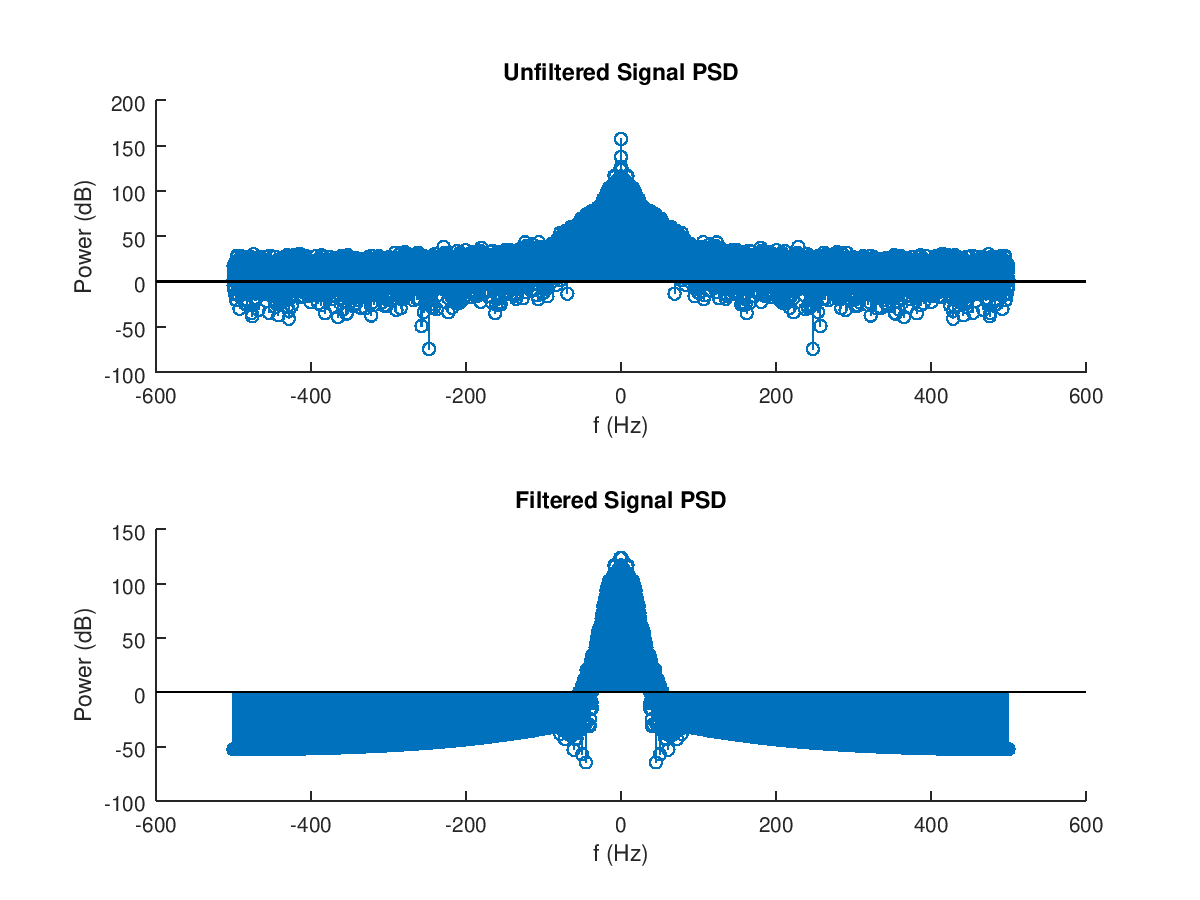
\includegraphics[scale=0.55]{figures/fig23-ecg2filteredpsd.png}}
\caption{PSD hasil proses \textit{filtering} terhadap sinyal sampel ECG 2}
\label{ecg2filteredpsd}
\end{figure}

Berbeda dengan sampel sebelumnya, PSD sampel ECG 2 tidak memiliki lonjakan daya yang terlihat pada frekuensi jala-jala dan harmonisanya, namun PSD sampel ECG 2 memiliki derau berfrekuensi rendah yang jauh lebih kuat dibandingkan sampel sebelumnya. Seperti pada sampel sebelumnya, setelah mengalami proses \textit{filtering}, berkat \textit{bandpass filter}, tampak bahwa derau berfrekuensi rendah mengalami peredaman dan memiliki daya yang wajar seperti pada frekuensi di sekitarnya. Daya yang sebelumnya tersebar pada seluruh rentang frekuensi pun kini menjadi terkonsentrasi pada rentang frekuensi sinyal ECG saja, yakni pada 0.5 Hz hingga 20 Hz seperti yang diharapkan. 

Dalam \textit{domain} waktu, perbedaan antara sinyal sampel ECG 2 mentah dengan sinyal hasil proses \textit{filtering} tampak jelas. Pada sinyal hasil proses \textit{filtering}, tidak terdapat pergeseran \textit{baseline} yang berarti dibandingkan dengan sinyal sampel mentah yang mengalami pergeseran \textit{baseline} yang ekstrem. Hal ini disebabkan komponen berfrekuensi rendah dari sinyal mentah telah diredam oleh \textit{bandpass filter}. Kemudian, \textit{jitter} yang muncul pada sinyal mentah pun tidak ditemukan pada sinyal hasil proses \textit{filtering}. Hal ini dikarenakan komponen berfrekuensi tinggi dari sinyal telah diredam pula oleh \textit{bandpass filter}, menyisakan komponen berfrekuensi dalam rentang frekuensi sinyal ECG, sehingga diperoleh bentuk sinyal ECG yang menyerupai \textit{template}. 

\begin{figure}[H]
\centerline{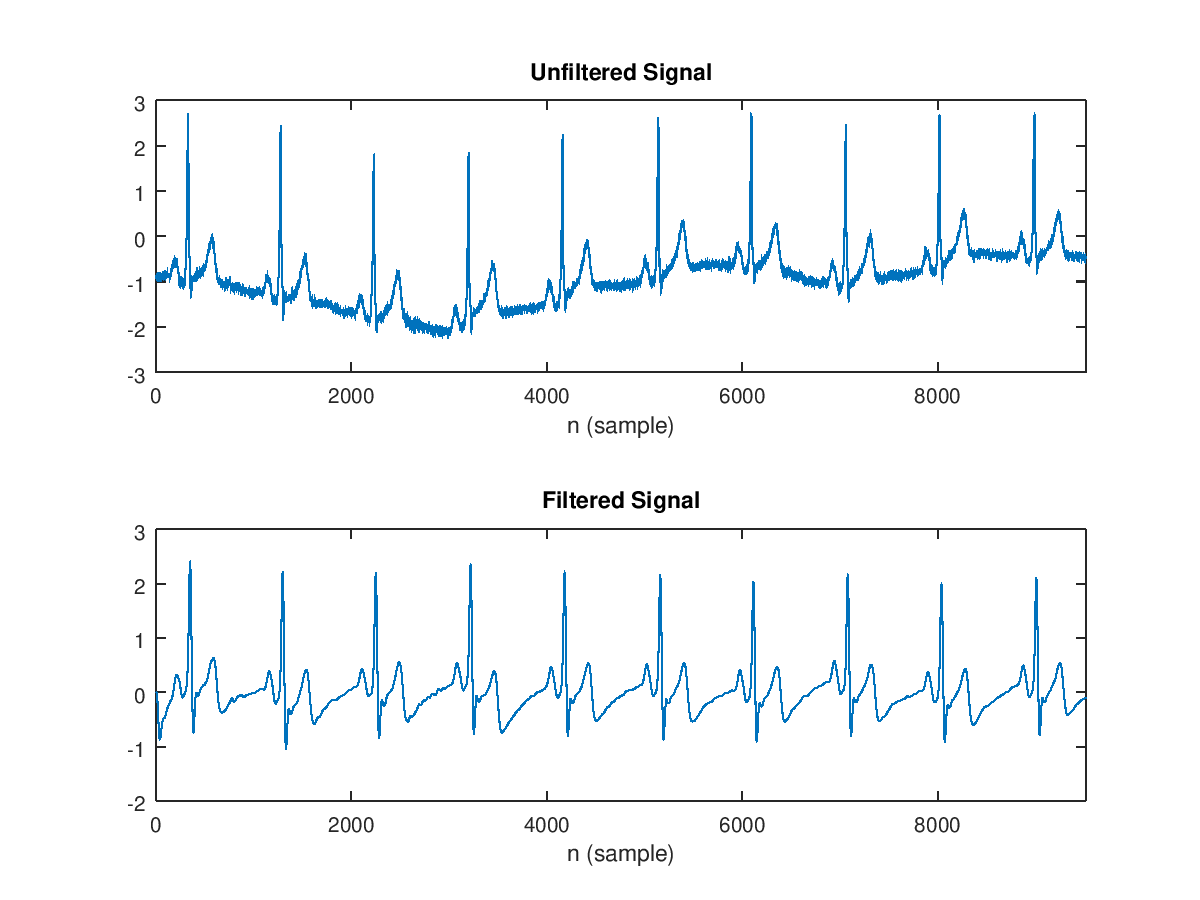
\includegraphics[scale=0.55]{figures/fig24-ecg2filteredtime.png}}
\caption{Hasil proses \textit{filtering} terhadap sinyal sampel ECG 2 dalam \textit{domain} waktu}
\label{ecg2filteredtime}
\end{figure}

\subsection{Kode}

Berikut adalah kode \textit{Octave} yang digunakan pada topik 2. Ketika dijalankan, kode ini akan menampilkan \textbf{pole-zero plot} filter yang digunakan, \textbf{respons frekuensi} filter yang digunakan, \textbf{PSD} sinyal sebelum dan sesudah proses \textit{filtering}, serta \textbf{sinyal dalam \textit{domain} waktu} sebelum dan sesudah proses \textit{filtering} dari kedua buah sinyal yang diberikan.

Kode ini menggunakan \textit{package} signal untuk menampilkan \textit{pole-zero plot} dari filter yang dirancang. Selain itu, kode ini tidak membutuhkan \textit{package} eksternal lainnya. Perancangan persamaan perbedaan dari \textit{comb filter} dan \textit{bandpass filter} pada kode ini diimplementasikan dengan fungsi buatan sendiri bernama \textbf{design\textunderscore comb}  dan \textbf{design\textunderscore butterworth\textunderscore bandpass}. Selain itu, kode ini menggunakan \textit{built-in function} \textbf{fft}, \textbf{fftshift}, \textbf{abs}, \textbf{unwrap}, \textbf{filter}, \textbf{freqz}, dan \textbf{conv}.

\lstinputlisting[caption={Kode \textit{Octave} untuk Topik 2: Sistem Sebagai Filter}]{octave_codes/topik_2.m}

\bibliographystyle{alpha}
\bibliography{references} % see references.bib for bibliography management

\end{document}
